	\documentclass[12pt]{article}
	\usepackage{hyperref}
	\usepackage{graphicx}
	\usepackage[T1]{fontenc}
	\usepackage[utf8]{inputenc}
	\usepackage{color}
	\usepackage[font=small,labelfont=bf]{caption}
	\usepackage[english]{babel}
	\usepackage{datetime}
	\usepackage{listings}
	\usepackage{fancyhdr}
	\usepackage{lastpage}
	\usepackage{float}
	\pagestyle{fancy}
	\fancyhf{}
	\usepackage{listings}
	\usepackage{color}
	\definecolor{lightgray}{rgb}{.9,.9,.9}
	\definecolor{darkgray}{rgb}{.4,.4,.4}
	\definecolor{purple}{rgb}{0.65, 0.12, 0.82}
	
	\lstdefinelanguage{JavaScript}{
		keywords={typeof, new, true, false, catch, function, return, null, catch, switch, var, if, in, while, do, else, case, break},
		keywordstyle=\color{blue}\bfseries,
		ndkeywords={class, export, boolean, throw, implements, import, this},
		ndkeywordstyle=\color{darkgray}\bfseries,
		identifierstyle=\color{black},
		sensitive=false,
		comment=[l]{//},
		morecomment=[s]{/*}{*/},
		commentstyle=\color{purple}\ttfamily,
		stringstyle=\color{red}\ttfamily,
		morestring=[b]',
		morestring=[b]"
	}
	
	\lstset{
		language=JavaScript,
		backgroundcolor=\color{lightgray},
		extendedchars=true,
		basicstyle=\footnotesize\ttfamily,
		showstringspaces=false,
		showspaces=false,
		numbers=none,
		numberstyle=\footnotesize,
		numbersep=9pt,
		tabsize=2,
		breaklines=true,
		showtabs=false,
		captionpos=b
	}
	
	\addtolength{\oddsidemargin}{-2.4cm}
	\addtolength{\evensidemargin}{-3cm}
	\addtolength{\textwidth}{5cm}
	\addtolength{\topmargin}{-3cm}
	\addtolength{\textheight}{5cm}
	\usepackage{multicol}
	\newcommand\textline[4][t]{%
		\par\smallskip\noindent\parbox[#1]{.333\textwidth}{\raggedright\texttt{}#2}%
		\parbox[#1]{.333\textwidth}{\centering#3}%
		\parbox[#1]{.333\textwidth}{\raggedleft\texttt{#4}}\par\smallskip%
	}
	\rfoot{\textline[t]{}{Page \thepage \hspace{1pt} of \pageref{LastPage}}{}}
	\renewcommand{\today}{\thisdayofweekname\ \the\day\ \monthname\ \the\year}
	\title{Essay}
	\date{}
	\author{Trevisan Davide}
	\hypersetup{
		colorlinks=true,       % false: boxed links; true: colored links
		linkcolor=blue,          % color of internal links (change box color with linkbordercolor)
		citecolor=green,        % color of links to bibliography
		filecolor=blue,      % color of file links
		urlcolor=blue,
		filecolor=red,
		citecolor=blue,
	}
	\begin{document}
		\pagenumbering{arabic}
		
		
		
		\begin{titlepage}
			
			\newcommand{\HRule}{\rule{\linewidth}{0.5mm}} % Defines a new command for the horizontal lines, change thickness here
			
			\center % Center everything on the page
			
			%----------------------------------------------------------------------------------------
			%	HEADING SECTIONS
			%----------------------------------------------------------------------------------------
			
			\textsc{\LARGE University of Padova}\\[1.5cm] % Name of your university/college
			\textsc{\Large Computer and Network Security}\\[0.5cm] % Major heading such as course name
			
			%----------------------------------------------------------------------------------------
			%	TITLE SECTION
			%----------------------------------------------------------------------------------------
			
			\HRule \\[0.4cm]
			{ \huge Privacy issues on Chrome extensions}\\[0.3cm]
			%Title of your document
			\HRule \\[1.5cm]
			
			%----------------------------------------------------------------------------------------
			%	AUTHOR SECTION
			%----------------------------------------------------------------------------------------
			
			\begin{minipage}{0.4\textwidth}
				\begin{flushleft} \large
					\emph{Students:}\\
					Davide Trevisan\\ % Your name
					Andrea Multineddu\\
				\end{flushleft}
			\end{minipage}
			~
			\begin{minipage}{0.4\textwidth}
				\begin{flushright}\large
					\emph{Registration number:} \\
					\textsc{1070686}\\ % matricola
					\textsc{1049261}\\
				\end{flushright}
			\end{minipage}\\[1cm]
			
			%----------------------------------------------------------------------------------------
			%	DATE SECTION
			%----------------------------------------------------------------------------------------
			
			{\large \today}\\[1cm] % Date, change the \today to a set date if you want to be precise
			
			%----------------------------------------------------------------------------------------
			%	LOGO SECTION
			%----------------------------------------------------------------------------------------
			
			
\includegraphics[scale=0.35]{Logo.png} % Include a department/university logo - this will require the graphicx package
			
			%----------------------------------------------------------------------------------------
			
			\vfill % Fill the rest of the page with whitespace
		\end{titlepage}
		
		\newpage

\begin{multicols}{2}
	\section*{Introduction}
	Nowadays the majority of browsers let users the possibility of customizing it in order to get a new feature or a new style of visualization to better match the taste of the single user.
	All of this is achievable through the existing extensions for modern browsers. But there is also the opposite situation in which a malicious user tries to get personal information using those extensions.
	
	\section*{Abstract}
	Google Chrome browser is known for it huge amount of extensions that let users do almost everything they want, but there are also malicious extensions that aim to steal personal information about the life, bank accounts and every other single piece of information of the users. In this paper we presents three extensions: ChromeLogger \cite{ChromeLogger}, Stealth Screenshot and Activity Logger;
	Our initial idea was to create a monitor for extension and integrate in ChromeLogger (that has a GNU license) other malicious functionalities. For this paper purpose we haven't touched the original ChromeLogger, but we developed an additional extension that aims to integrate with it: In  fact only few modifications to the manifest are needed, because all of the code is developed as listeners and is very portable. A simple example of the fusion of the two apps can be found \href{https://github.com/Trexy94/Fusion}{here}.
	\paragraph{}ChromeLogger is a keylogger and form grabber for Google Chrome that runs as an extension.	
	ChromeLogger works by injecting javascript into all loaded web pages. This extension hasn't been developed by us, but we want to talk about it because the way this extension works is very interesting and it is a serious threat.
	\paragraph{}Stealth Screenshot makes screenshots of the active tab based on a timer and keep them until every opened tab is closed. Users can access with a combination of key to all screenshots taken during the session, keeping a log of the sites.
	\paragraph{}Activity Logger keeps trace of all events related to extension and save them in Chrome storage. Users can check if there are installation, uninstallation, activation or deactivation of Chrome extension due to malicious code running in background.
	\paragraph{}All extensions works on the last version of Chrome (at the moment 52.0.2743.116 m).
	\section*{Related work}
	There is obviously some literature about how chrome extension works: an interesting job in evaluating the security architecture and recommendation for security improvement has been done by Nicholas Carlini et al. \cite{Carlini}. An other interesting Job on evaluating malicious extensions has been done by Nav Jagpal et al. \cite{Nav}, that is an evolution of HULK \cite{HULK}. An interesting job on analysis of malicious javascript code has been done by Mohan Dhawan and Vinod Ganapathy \cite{Java}
	We have found more easy to understand to talk about each extension related works separately.
\section*{How Chrome Extension works}
\subsection*{Background}
\subsubsection*{where to find an extension}
The Chrome Web Store is the official way for users
to find and install extensions, where the developers can publish it. They can also push out updates without any action
by the end-user.
In addition to the Chrome Web Store, extensions can
also be installed manually by a user or an external program.
Extension that are not downloaded through the official channel are flagged by Chrome when it starts	and the user is asked to disable them.
However, the user can whitelist the extension through the console.
\subsubsection*{Manually install an extension}
	Once you have all the source code of an extension in a folder, go to  \textsc{chrome://extensions} (or find it in the menu in more tools > extensions), then activate the developer mode on the top right of the page. To install the extension, you just have to indicate where is the folder on your computer after clicking on load unpacked extension. For \textsc{.crx} packaged extension, you have to drag them on the \textsc{chrome://extensions} tab and then confirm that you want to install it (it's not directly possible because of the stronger security policy of Chrome)
\subsection*{Permissions}
Chrome requires extensions to list the
permissions needed to access the different parts of the
extension API. The complete list of the permissions and their interaction can be retrieved on Google developer page \cite{Google}.
\paragraph{}Extensions must also specify a list of content scripts to indicate
JavaScript files that will run inside of the web page, because this is a powerful feature that allows an extension to be indistinguishable to the web page behavior. Besides the content scripts that
allow an extension to interact with a given page,
Chrome also allows extensions to run scripts in a
“background page” that often contain the
logic and state an extension needs for the entirety
of the browser session and do not have any visibility
to the user.For example this is the manifest of the stealth screenshot extension:
\begin{lstlisting}
{
"name": "Stealth Screenshot Extension",
"version": "0.1",
"description": "This is a prototype
 of a background screenshot extension",
"background": {
"persistent": true,
"scripts": ["background.js"]
},
"commands": {
"toggle": {
"suggested_key": {
"windows": "Ctrl+Shift+Y",
"mac": "Command+Shift+Y",
"chromeos": "Ctrl+Shift+U",
"linux": "Ctrl+Shift+J"
},
"description": "My description"
}
},
"browser_action": {
"default_icon": "camera.png",
"default_title": "Take a screen shot!"
},
"omnibox": { "keyword" : "show" },
"permissions": [
"storage",
"tabs",
"<all_urls>",
"unlimitedStorage",
"activeTab"
],
"manifest_version": 2
}
\end{lstlisting}
as you can see, an extension has to declare in addition to all the permissions and all the interaction it has with the user such as an input in the omnibox or the click on the icon.
\section*{Activity Logger Extension}
The source code of the extension (not fully functional) we developed is downloadable \href{https://github.com/andreamultineddu/Activity-Logger}{here}
\subsection*{Related work}
On the Chrome Web Store i haven't found any extension that is similar to the one we are presenting.
A motivation of the absence of similar works can possibly found in the Chrome API that are really poor in terms of functionality and can result in lack of interest to patch security issue coming from the use of extensions. If in near future, Google decides to increase the functionality of his API in the extensions management maybe could appear some interesting solution in this field.
\subsection*{Scope of the extension}
The extension aims to keep traces about the activities of other extensions and let the user know
about them through a dedicate page in which can check for every extension that are installed on the
Chrome browser. This logger keep traces of logs even if some extensions are uninstalled. \\
The extension makes use of the following permission the manifest file:
\begin{itemize}
	\item  management
	\item  storage
	\item  unlimitedStorage
\end{itemize}
\subsection*{How the extension work}
The extension at the browser start check the list of installed extension and updates the logs list with the one missing from it.
After this first check and update we create listener for the events related to extensions which are: 
\begin{itemize}
	\item  chrome.management.onInstalled
	\item  chrome.management.onUninstalled
	\item  chrome.management.onEnabled
	\item  chrome.management.onDisabled
\end{itemize}
Every time the user or some malicious code install, uninstall, enable or disable an extension a log of the triggered event is saved in the specific event log for the specific extension in the Chrome storage.
The computation time is defined by the computation time of the Chrome search in his storage.
\subsection*{Performance}
There aren't expensive operations or recursive function calls that requires a lot of computation so we can state that the impact on the CPU is negligible.
\subsection*{Limitations}
The main limitation of this extension can be reconducted to the limitation imposed by or to the absence of Chrome APIs.
At the moment we can just check the events described early in the paper, every other event defined in Chrome APIs and the presence or the absence of listener for a specific event.
A better control on browser activity could be achieved by adding APIs, for example that return the name of extension from which is running codes in response to a specific event.
\subsection*{Future work}
The final aims of this extension are to log every single activity of installed extensions and jasvacript scripts inside web pages in response to every event happening inside Chrome itself (like a modification inside the Chrome storage area) or the web pages visited by the user (the pressure of a button) and let the user check these logs	in order to let users check some strange and unwanted activities caused by some malicious code. At this time, for what we have find out from our research on Chrome API documentation we can just check if there is some code waiting a specific events that trigger it.
But this is also a double-edged weapon that can led to problems for privacy maintenance because let every user, capable of writing Chrome extension the possibility to check every activity, but from the other hands let malicious users the possibility  on customizable browsers to get knowledge about users routines, personal data and ad-hoc javascript code injection.
\section*{ChromeLogger}
There are other keylogger and form grabber, but we chose to take this extension as a base for many reasons:
\begin{itemize}
	\item It is in an open license, so we can modify it and use the code as we like.
	\item It is a chrome extension, and it needs no other support application (this has some limitations on the data it can collect, but we wanted to see how malicious can be a pure chrome extension).
	\item It is a simple, but effective, keylogger and form grabber, so we can use a easy to understand base.
	\item Differently to normal keyloggers, this solution is not considered as a threat by the OS.
\end{itemize} 
\subsection*{Scope of the extension}
The extension is a form grabber for Google Chrome running natively in it without the need to install additional external software. It works on every loaded web pages acting on every form in the pages.
The extension manages to let the user check, for every submitted form, all the keystrokes done and some additional data about the time of submission. This is done by an additional page where is possible to turn on some additional option for the form grabber and visualize all the data collected by the extension.
The extension makes use of the following permissions in the manifest file:
\begin{itemize}
	\item  <all\_urls>
	\item  tabs
	\item  storage
	\item  unlimitedStorage
\end{itemize}
\subsection*{How the extension work}
When a web page is completely loaded ChromeLogger injects javascript in it. The payload records keypresses using event listeners and saves them to Chrome's storage. Unlike other browser keyloggers, ChromeLogger runs natively in Chrome (on all OS's) without the need to install additional software.
The form grabber works in a similar way. Javascript is injected and event listeners are added for all forms. When a form is submitted, its data is saved to ChromeLogger's storage. This allows form data transferred over SSL to be saved in plaintext.
ChromeLogger's payload is written in pure JS and the log viewer is built using AngularJS. When a form is submitted, its data is saved to ChromeLogger's storage with the add of URL and time data about the submission of the form.
The user has also access to an option page where he can turn on or off some optional features and check all the logs inside a table where can filtering and ordering them by the data and URL.
\subsubsection*{Injection}
The injection is simple but effective:
\begin{lstlisting}
chrome.tabs.onUpdated.addListener(function(tabId, changeInfo) {
if (changeInfo.status === 'complete') {
chrome.tabs.executeScript(tabId, {
allFrames: true, 
file: 'src/inject/payload.js'
});
}
});
\end{lstlisting}
this allows the extension to add to the standard javascript of the page a malign javascript that allows the extension to receive and save all the form submitted by user and also the message submitted through social apps (for example whatsapp web)
\subsection*{Performance}
There aren't expensive operations or recursive function calls that requires a lot of computation so we can state that the impact on the CPU is negligible.
\section*{Stealth Screenshot Extension}
The source code of the extension we developed is downloadable \href{https://github.com/Trexy94/Stealth-screenshot}{here}. The aim of the stealth screenshot extension is to create a small prototype of an extension that catch screenshots at a regular interval with the minimum possible user interaction and obviously giving back the screenshot acquired and a log of the sites visited. In this case the extension is stealthed like a normal simple screenshot extension.
\subsection*{Related work}
For the visited website logging there are a lot of apps on the store that do the same action, obviously not for malicious interests.
For the screenshots collection, i haven't found any extension that works in the same way: most common screenshots extensions allows the user to schedule a succession of screenshots. But the extension we propose aims to do it without user consensus, and it's a big difference.
For the development of this app we made no use of existing works, we used only Google APIs documentation \cite{GoogleDoc}. There aren't in the literature we searched in no similar works, probably for the very limitative threat model, that presumes that you can have access to a target PC at a regular interval. However, we think that this type of attack can be an issue for example in work places. Also, if we will be able to do some improvements to the code, this can be a serious threat.
\subsection*{How the extension work}
\subsubsection*{Activation and screenshot collection}
The extension uses the relatively new tab APIs given by Chrome too take screenshot.
The extension makes use of the following permissions:\begin{itemize}
	\item storage
	\item tabs
	\item <all\_urls>
	\item unlimited storage
	\item active tab
	\end{itemize}
	This is the core part of the extension:
	\begin{lstlisting}
var imglist=[];
.............................
// Listen for a click on the camera icon. On that click, take a screenshot.
chrome.browserAction.onClicked.addListener(function() {
chrome.windows.create({type: "popup",state:"minimized"})//the idea is this new window keeps alive chrome and screenshots, offering something interesting to the user.
interval=0;
while(interval<30000000)//print x times, where x is the number of milliseconds/milliseconds for screenshot
{
setTimeout(function(){Loop()},interval);    
interval=interval+60000;
}
});

function Loop (){
chrome.tabs.captureVisibleTab(function(screenshotUrl) {
imglist[index]=screenshotUrl;
chrome.tabs.getSelected(null, function(tab) {list=list+tab.url+"----"+new Date().toJSON()+"\n";});
index++;
if (chrome.runtime.error) {
console.log("Runtime error.");
}
}); 
chrome.storage.local.set({"lista": list});

}
............................
	\end{lstlisting}
	 The extension works in a simple way: it triggers on a browser event, in this case the click on the icon of the extension, but there are other possibilities: we tested that there are no simple ways to take screenshot with no interaction, because the security policy of the API doesn't allow to take a screenshot without some kind of events, presuming that the user should be aware of what is happening; not triggering any event returns only null.
Once triggered, the extension schedule all the future screenshot through the Javascript setTimeout method: this allows to take screenshot for hours, with only the need for a click to start.
The screenshot are stored in an array visible to all the extension methods.
In addition a log of all the pages that were active when the screenshot was taken is saved, and stored locally. So we can try to spoof the \textsc{GET} request done by the user.
\subsubsection*{Screenshot retrieval}
The screenshot can be collected in two ways in the extension we developed:
through a combination of key for retrieving all screenshots (we programmed it on Ctrl+Shift+Y) or writing "show" in the omnibox, pressing "tab" and writing in the omnibox the number of screenshot to show (starting from the last one). Writing "list" instead opens a popup with the log of the sites.
 The log is persistent; in this prototype we chose to keep only the list of the sites in the last session, but it can be easily modified to not lose any data as it is been done in the fusion with ChromeLogger, for example.
\subsubsection*{Performance}
We tested that the extension is able to take screenshot with a interval of 1 minute for more than 2 hours without losing any screenshot.
The application occupy less of 50MB of RAM for an hour of screenshots taken every minute. The impact on the CPU is negligible.
Screenshot retrieval through the key combo however can crash Chrome, although it never happened in our PC because of the great performance (we had an Intel i5 6400, with 8GB of DDR4 memory and SSD), but it got frozen for some seconds.
\subsection*{Limitations}
The major limitation of this extension is that the screenshots only live until the extension is active: this implies that closing all the windows of Chrome completely deletes the screenshot taken.
This is a consequence of how the API and the Chrome sandbox works. At the moment, we found no way to get around it, but we are pretty much confident that is possible to save those screenshots, but due to our lack of knowledge we are not able at the moment to demonstrate it.
\subsection*{Future work}
Possible future works will focus on find a way to save those screenshot.
The application should also be rewritten without the tab API, to avoid of the limitation of it.
Javascript inject the code for the screenshot or use it for simulate the right events should do the work, but the time and the train needed to do it made impossible for us to test it for this paper.
\section*{Conclusions}
\begin{figure}[H]
	\begin{center}
		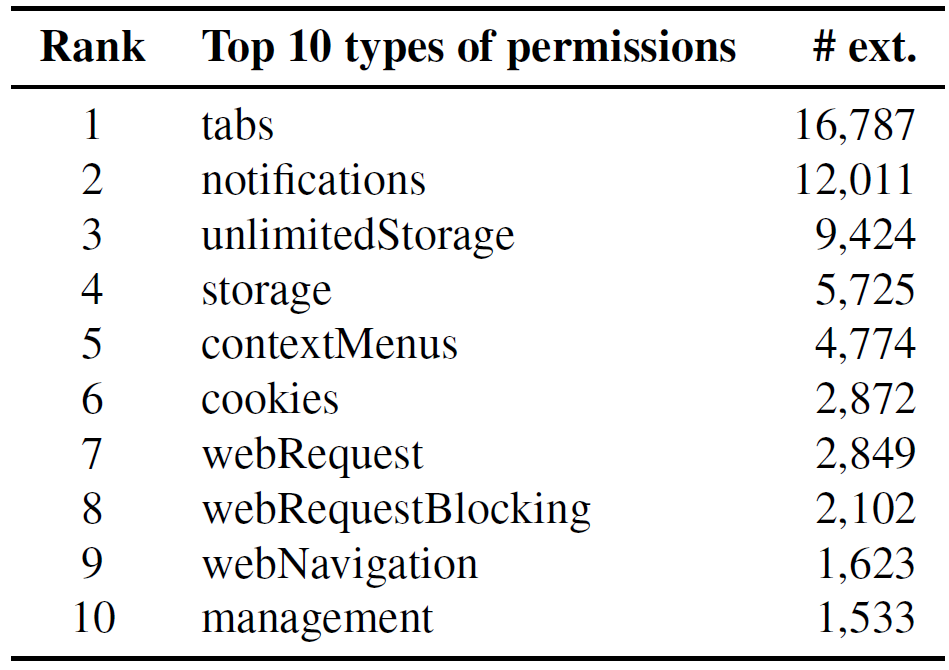
\includegraphics[width=9cm]{permission.png}
		\caption{The top 10 permissions found in the manifest
			files for all extensions HULK ran. Extensions can include			
			more than one permission.}
	\end{center}
\end{figure}
Chrome should improve their task manager, to give the users more knowledge about what is happening in their PC, because is possible to create a timed or a smart bomb with a simple \textsc{while(true)} cycle, and it can crash Chrome, because the sandbox sometimes can't handle it.
All the solution we have presented in this paper makes use of the most used Chrome permission, as already stated in the HULK paper \cite{HULK}
As shown in the screenshot extension, taking screenshot without user consensus should not be allowed to the API (just a popup should be enough). \\
The ChromeLogger and Stealth Screenshot show the presence of issues regarding the maintenance of user's privacy, and the Activity Logger can be used as a little warden against unwanted modification of extensions list. We still find out ways to bring Google Chrome to crash in a really simple way using the basics keyword of Javascript.

\begin{thebibliography}{8}
	\bibitem{Google}
	Google developer page-permissions
	\href{https://developer.chrome.com/extensions/declare_permissions}{https://developer.chrome.com/extensions/\\declare\_permissions}
	
	\bibitem{GoogleDoc}
	Google developer page-API
	\href{https://developer.chrome.com/extensions/api_index}{https://developer.chrome.com/extensions/\\api\_index}
	
	\bibitem{ChromeLogger}
	Eric Zhang,\\
	\emph{ChromeLogger},\\
A keylogger and form grabber for Google Chrome that runs as an extension.\\
\href{https://github.com/Xeroday/ChromeLogger}{ChromeLogger}\\
\href{https://www.ericzhang.me/projects/chromelogger/}{referring site}

\bibitem{HULK}
\emph{Hulk: Eliciting Malicious Behavior in Browser Extensions}\\
Alexandros Kapravelos, Chris Grier, Neha Chachra, Christopher Kruegel
Giovanni Vigna, Vern Paxson,
UC Santa Barbara,
UC Berkeley, 
UC San Diego and 
International Computer Science Institute\\
\emph{23rd USENIX Security Symposium.}\\
\href{https://www.usenix.org/system/files/conference/usenixsecurity14/sec14-paper-kapravelos.pdf}{Paper}\\

\bibitem{Carlini}
\emph{An Evaluation of the Google Chrome Extension Security Architecture}\\
Nicholas Carlini, Adrienne Porter Felt, and David Wagner\\
\emph{21st USENIX Security Symposium.}\\
\href{https://www.usenix.org/system/files/conference/usenixsecurity12/sec12-final177_0.pdf}{Paper}

\bibitem{Nav}
\emph{Trends and Lessons from Three Years Fighting
	Malicious Extensions}\\
Nav Jagpal, Eric Dingle, Jean-Philippe Gravel, Panayiotis Mavrommatis,
Niels Provos, Moheeb Abu Rajab, and Kurt Thomas, Google\\
\emph{24th USENIX Security Symposium}
\href{https://www.usenix.org/system/files/conference/usenixsecurity15/sec15-paper-jagpal.pdf}{Paper}
\bibitem{Java}
\emph{Analyzing Information Flow in JavaScript-based Browser Extensions}\\
Mohan Dhawan and Vinod Ganapathy\\
Department of Computer Science, Rutgers University\\
\emph{Proc. of Annual
	Computer Security Applications Conference, 2009}
\href{https://www.acsac.org/2009/openconf/modules/request.php?module=oc_program&action=view.php&id=10}{Paper}
\end{thebibliography}
\end{multicols}
 
\end{document}
